\documentclass[conference]{IEEEtran}
% *** MISC UTILITY PACKAGES ***
%\usepackage{ifpdf}
% Heiko Oberdiek's ifpdf.sty is very useful if you need conditional
% compilation based on whether the output is pdf or dvi.
% usage:
% \ifpdf
%   % pdf code
% \else
%   % dvi code
% \fi
% The latest version of ifpdf.sty can be obtained from:
% http://www.ctan.org/pkg/ifpdf
% Also, note that IEEEtran.cls V1.7 and later provides a builtin
% \ifCLASSINFOpdf conditional that works the same way.
% When switching from latex to pdflatex and vice-versa, the compiler may
% have to be run twice to clear warning/error messages.

% *** GRAPHICS RELATED PACKAGES ***
\ifCLASSINFOpdf
   \usepackage[pdftex]{graphicx}
   \usepackage{amsfonts}
   \usepackage{bbding}
   \usepackage{pifont}
  % declare the path(s) where your graphic files are
   \graphicspath{{../pdf/}{../jpeg/}}
  % and their extensions so you won't have to specify these with
  % every instance of \includegraphics
   \DeclareGraphicsExtensions{.pdf,.jpeg,.png}
\else
  % or other class option (dvipsone, dvipdf, if not using dvips). graphicx
  % will default to the driver specified in the system graphics.cfg if no
  % driver is specified.
   \usepackage[dvips]{graphicx}
   \usepackage{tikz}
   \usepackage{amsfonts}
  % declare the path(s) where your graphic files are
   \graphicspath{{../eps/}}
  % and their extensions so you won't have to specify these with
  % every instance of \includegraphics
   \DeclareGraphicsExtensions{.eps}
\fi
% graphicx was written by David Carlisle and Sebastian Rahtz. It is
% required if you want graphics, photos, etc. graphicx.sty is already
% installed on most LaTeX systems. The latest version and documentation
% can be obtained at:
% http://www.ctan.org/pkg/graphicx
% Another good source of documentation is "Using Imported Graphics in
% LaTeX2e" by Keith Reckdahl which can be found at:
% http://www.ctan.org/pkg/epslatex
%
% latex, and pdflatex in dvi mode, support graphics in encapsulated
% postscript (.eps) format. pdflatex in pdf mode supports graphics
% in .pdf, .jpeg, .png and .mps (metapost) formats. Users should ensure
% that all non-photo figures use a vector format (.eps, .pdf, .mps) and
% not a bitmapped formats (.jpeg, .png). The IEEE frowns on bitmapped formats
% which can result in "jaggedy"/blurry rendering of lines and letters as
% well as large increases in file sizes.
%
% You can find documentation about the pdfTeX application at:
% http://www.tug.org/applications/pdftex

% *** MATH PACKAGES ***
%
\usepackage{amsmath}
\usepackage{pifont}
% A popular package from the American Mathematical Society that provides
% many useful and powerful commands for dealing with mathematics.
%
% Note that the amsmath package sets \interdisplaylinepenalty to 10000
% thus preventing page breaks from occurring within multiline equations. Use:
%\interdisplaylinepenalty=2500
% after loading amsmath to restore such page breaks as IEEEtran.cls normally
% does. amsmath.sty is already installed on most LaTeX systems. The latest
% version and documentation can be obtained at:
% http://www.ctan.org/pkg/amsmath

% *** ALIGNMENT PACKAGES ***
%
\usepackage{array}
% Frank Mittelbach's and David Carlisle's array.sty patches and improves
% the standard LaTeX2e array and tabular environments to provide better
% appearance and additional user controls. As the default LaTeX2e table
% generation code is lacking to the point of almost being broken with
% respect to the quality of the end results, all users are strongly
% advised to use an enhanced (at the very least that provided by array.sty)
% set of table tools. array.sty is already installed on most systems. The
% latest version and documentation can be obtained at:
% http://www.ctan.org/pkg/array


% IEEEtran contains the IEEEeqnarray family of commands that can be used to
% generate multiline equations as well as matrices, tables, etc., of high
% quality.

% *** SUBFIGURE PACKAGES ***
\ifCLASSOPTIONcompsoc
  \usepackage[caption=false,font=normalsize,labelfont=sf,textfont=sf]{subfig}
\else
  \usepackage[caption=false,font=footnotesize]{subfig}
\fi
% subfig.sty, written by Steven Douglas Cochran, is the modern replacement
% for subfigure.sty, the latter of which is no longer maintained and is
% incompatible with some LaTeX packages including fixltx2e. However,
% subfig.sty requires and automatically loads Axel Sommerfeldt's caption.sty
% which will override IEEEtran.cls' handling of captions and this will result
% in non-IEEE style figure/table captions. To prevent this problem, be sure
% and invoke subfig.sty's "caption=false" package option (available since
% subfig.sty version 1.3, 2005/06/28) as this is will preserve IEEEtran.cls
% handling of captions.
% Note that the Computer Society format requires a larger sans serif font
% than the serif footnote size font used in traditional IEEE formatting
% and thus the need to invoke different subfig.sty package options depending
% on whether compsoc mode has been enabled.
%
% The latest version and documentation of subfig.sty can be obtained at:
% http://www.ctan.org/pkg/subfig

% *** FLOAT PACKAGES ***
%
%\usepackage{fixltx2e}
% fixltx2e, the successor to the earlier fix2col.sty, was written by
% Frank Mittelbach and David Carlisle. This package corrects a few problems
% in the LaTeX2e kernel, the most notable of which is that in current
% LaTeX2e releases, the ordering of single and double column floats is not
% guaranteed to be preserved. Thus, an unpatched LaTeX2e can allow a
% single column figure to be placed prior to an earlier double column
% figure.
% Be aware that LaTeX2e kernels dated 2015 and later have fixltx2e.sty's
% corrections already built into the system in which case a warning will
% be issued if an attempt is made to load fixltx2e.sty as it is no longer
% needed.
% The latest version and documentation can be found at:
% http://www.ctan.org/pkg/fixltx2e

%\usepackage{stfloats}
% stfloats.sty was written by Sigitas Tolusis. This package gives LaTeX2e
% the ability to do double column floats at the bottom of the page as well
% as the top. (e.g., "\begin{figure*}[!b]" is not normally possible in
% LaTeX2e). It also provides a command:
%\fnbelowfloat
% to enable the placement of footnotes below bottom floats (the standard
% LaTeX2e kernel puts them above bottom floats). This is an invasive package
% which rewrites many portions of the LaTeX2e float routines. It may not work
% with other packages that modify the LaTeX2e float routines. The latest
% version and documentation can be obtained at:
% http://www.ctan.org/pkg/stfloats
% Do not use the stfloats baselinefloat ability as the IEEE does not allow
% \baselineskip to stretch. Authors submitting work to the IEEE should note
% that the IEEE rarely uses double column equations and that authors should try
% to avoid such use. Do not be tempted to use the cuted.sty or midfloat.sty
% packages (also by Sigitas Tolusis) as the IEEE does not format its papers in
% such ways.
% Do not attempt to use stfloats with fixltx2e as they are incompatible.
% Instead, use Morten Hogholm'a dblfloatfix which combines the features
% of both fixltx2e and stfloats:
% \usepackage{dblfloatfix}
% The latest version can be found at:
% http://www.ctan.org/pkg/dblfloatfix

% *** PDF, URL AND HYPERLINK PACKAGES ***
%
\usepackage{url}
\usepackage{tabu}
% url.sty was written by Donald Arseneau. It provides better support for
% handling and breaking URLs. url.sty is already installed on most LaTeX
% systems. The latest version and documentation can be obtained at:
% http://www.ctan.org/pkg/url
% Basically, \url{my_url_here}.

% *** Do not adjust lengths that control margins, column widths, etc. ***
% *** Do not use packages that alter fonts (such as pslatex).         ***
% There should be no need to do such things with IEEEtran.cls V1.6 and later.
% (Unless specifically asked to do so by the journal or conference you plan
% to submit to, of course. )

% An example of a floating figure using the graphicx package.
% Note that \label must occur AFTER (or within) \caption.
% For figures, \caption should occur after the \includegraphics.
% Note that IEEEtran v1.7 and later has special internal code that
% is designed to preserve the operation of \label within \caption
% even when the captionsoff option is in effect. However, because
% of issues like this, it may be the safest practice to put all your
% \label just after \caption rather than within \caption{}.
%
% Reminder: the "draftcls" or "draftclsnofoot", not "draft", class
% option should be used if it is desired that the figures are to be
% displayed while in draft mode.
%

% Note that the IEEE typically puts floats only at the top, even when this
% results in a large percentage of a column being occupied by floats.

% An example of a double column floating figure using two subfigures.
% (The subfig.sty package must be loaded for this to work.)
% The subfigure \label commands are set within each subfloat command,
% and the \label for the overall figure must come after \caption.
% \hfil is used as a separator to get equal spacing.
% Watch out that the combined width of all the subfigures on a
% line do not exceed the text width or a line break will occur.
%
%\begin{figure*}[!t]
%\centering
%\subfloat[Case I]{\includegraphics[width=2.5in]{box}%
%\label{fig_first_case}}
%\hfil
%\subfloat[Case II]{\includegraphics[width=2.5in]{box}%
%\label{fig_second_case}}
%\caption{Simulation results for the network.}
%\label{fig_sim}
%\end{figure*}
%
% Note that often IEEE papers with subfigures do not employ subfigure
% captions (using the optional argument to \subfloat[]), but instead will
% reference/describe all of them (a), (b), etc., within the main caption.
% Be aware that for subfig.sty to generate the (a), (b), etc., subfigure
% labels, the optional argument to \subfloat must be present. If a
% subcaption is not desired, just leave its contents blank,
% e.g., \subfloat[].

% An example of a floating table. Note that, for IEEE style tables, the
% \caption command should come BEFORE the table and, given that table
% captions serve much like titles, are usually capitalized except for words
% such as a, an, and, as, at, but, by, for, in, nor, of, on, or, the, to
% and up, which are usually not capitalized unless they are the first or
% last word of the caption. Table text will default to \footnotesize as
% the IEEE normally uses this smaller font for tables.
% The \label must come after \caption as always.
%
%\begin{table}[!t]
%% increase table row spacing, adjust to taste
%\renewcommand{\arraystretch}{1.3}
% if using array.sty, it might be a good idea to tweak the value of
% \extrarowheight as needed to properly center the text within the cells
%\caption{An Example of a Table}
%\label{table_example}
%\centering
%% Some packages, such as MDW tools, offer better commands for making tables
%% than the plain LaTeX2e tabular which is used here.
%\begin{tabular}{|c||c|}
%\hline
%One & Two\\
%\hline
%Three & Four\\
%\hline
%\end{tabular}
%\end{table}
\newcommand{\xmark}{\text{\ding{55}}}
% Note that the IEEE does not put floats in the very first column
% - or typically anywhere on the first page for that matter. Also,
% in-text middle ("here") positioning is typically not used, but it
% is allowed and encouraged for Computer Society conferences (but
% not Computer Society journals). Most IEEE journals/conferences use
% top floats exclusively.
% Note that, LaTeX2e, unlike IEEE journals/conferences, places
% footnotes above bottom floats. This can be corrected via the
% \fnbelowfloat command of the stfloats package.

% For peer review papers, you can put extra information on the cover
% page as needed:
% \ifCLASSOPTIONpeerreview
% \begin{center} \bfseries EDICS Category: 3-BBND \end{center}
% \fi
%
% For peerreview papers, this IEEEtran command inserts a page break and
% creates the second title. It will be ignored for other modes.

% correct bad hyphenation here
\hyphenation{op-tical net-works semi-conduc-tor}

\begin{document}
\title{\textit{Traffic Management Systems for Congestion Control and Collision Avoidance
in Smart City: A Survey}}

% author names and affiliations
\author{\IEEEauthorblockN{Mohaminul Alam}
\IEEEauthorblockA{University of Ottawa\\
malam096@uottawa.ca}
\and
\IEEEauthorblockN{Suranjit Banik}
\IEEEauthorblockA{University of Ottawa\\
Sbani041@uOttawa.ca}}

% make the title area
\maketitle

\begin{abstract}
%Refresh this?
Traffic Management systems (TMS) subjects have been handled since long time, fundamentally by structural architects and by city organizers. The presentation of new correspondence innovations - for example, Global Positioning Systems (GPS), cell networks and vehicle to vehicle communication has fundamentally changed the way analysts manage TMS issues. In this survey, we give an audit and a characterization of how TMS has been tended to in the writing. We begin from the current accomplishments of standard ways to deal with urban traffic estimation and enhancement, including strategies in light of the investigation of information gathered by settling sensors (e.g., cameras and radars), and techniques in light of data gave by cell phones, for example, Floating Car Data (FCD). A while later, we point out important issues form recent research paper related to urban traffic system, advancement, traffic light control and congestion control etc. At that point, in the wake of reviewing the fundamental ideas of traffic management system we concentrate on V2V and V2I communication and survey on latest proposed technologies.This survey aims to address latest strides in both infrastructure-free mechanism and infrastructure-based methodologies in TMS. 
\end{abstract}

\begin{IEEEkeywords}
Survey; Smart Signal; Smart City; Wireless Sensor Network (WSN); sensor; traffic management; Congestion control;
\end{IEEEkeywords}
% no keywords

\IEEEpeerreviewmaketitle

\section{Introduction}
In this day and age, everybody covet for a quick paced life even without pestering for the human life. These days because of less demanding EMI choices individuals can bear the cost of extravagance autos, bicycles hence adding to the movement step by step. Indeed, even producers have embraced different promoting systems like how much mileage a vehicle provides for increment the deals. This adds to the activity pledges as well as expands the danger of passing because of accidents and vehicle crash.
The fundamental thought of IoT is unavoidably furnishing us with an assortment of things or items, for example, radio frequency identification (RFID) labels, sensors, actuators, and cell phones, which can connect and coordinate with each other to do the errands of correspondence, calculation, and administration \cite{Multimedia:chao}. Such a system puts a splendid closer view for expanded information, mixed media applications as interest for rising applications like video on request (VoR), IPTV, and voice over IP (VoIP) has developed massively \cite{SecuringCloudServers:Chapade}. Figure 1 gives a complete case of sight and sound administration, engineering with regards to IoT \cite{Multimedia:chao}.
  
  TMS are made by a set out of utilization and management devices to incorporate correspondence, sensing and handling innovations. In outline, TMS collect movement related information from heterogeneous sources such as vehicles, activity lights, in-street and roadside sensors and so on. Besides, by totaling and exploiting such activity related information into an agreeable way (e.g. among vehicles)  \cite{VehicularNetworking:Karagiannis}  or into a Traffic Management Center(TMC) moved in a Cloud or in a Data center,several activity perils can be distinguished and consequently controlled enhancing the general activity productivity and providing a smooth movement flow.
  
  Within TMS, one building hinder that makes it is the Vehicular Ad hoc Networks (VANET), which provides data trade between vehicles, roadside units (RSU) and TMC. Detailed about road RSU and TMC will be discussed in section III. In VANETs, vehicles are portable hubs with an On-board Unit (OBU) that has installed sensors,processing units and remote interfaces in which vehicles can convey among themselves to make a ad-hoc network \cite{2012efficient:villas}.
\begin{figure}[!htb]
\centering
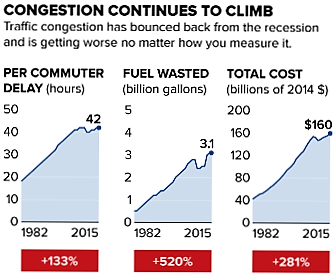
\includegraphics[width=3.5in]{statistics}
\caption{2105 urban mobility scoreboard in USA}
\label{Statistics_in _USA}
\end{figure} 
  However, packing in managing the traffic congestion starting point and in tending to its related problems, several TMS's have been proposed concentrating on adjust the speed of the vehicles keeping in mind the end goal to lessen the time spent in traffic lights, The average delay per traveler is more than twice what it was in the early 1980s. According to Inrix and TTI\footnote{http://abcnews.go.com/US/time-americans-waste-traffic/story?id=33313765} shows in Figure\ref{Statistics_in _USA}, without “more assertive approaches on the project, program, and policy fronts,” congestion will mostly only get worse.
 
 \subsection{Motivation and Scope}
  By considering residents' life, the urban planning and smart city applications have significant effects, which incorporate the impact on the national as far as wellbeing and security, catastrophe administration, pollution control, thus on so forward. Sensors service are being used for various projects identified with checking of cyclist, autos, public auto parking, and so on for the accumulation of particular space information. Evidently, unique other administration area applications are recognized that uses smart city IoT foundation to arrangement operations in air, noise, pollution, and observation framework in the urban communities.

Recent research published by a couple of Toronto designers think they have an answer for intelligent traffic management systems. The University of Toronto educator and PhD understudy have concocted an activity light which utilizes computerized reasoning to speed things up (in review paper by El-Tantawy \textit{et al.}\cite{el-trantaway:multiagent} and global-recognition\footnote{http://www.utoronto.ca/news/smarter-traffic-lights-win-global-recognition-u-t-grad}). A virtual test on 60 Toronto crossing points found the framework, named MARLIN, could slice hold up times by up to 40 for each penny. Both scholastic and regions are paying heed. Samah El-Tantawy said she was enlivened to take a shot at the venture by observing the effect of roads turned parking lots in Toronto and the place where she grew up, Cairo, Egypt. Right now most traffic lights are controlled by clocks or they utilize sensors snared to a concentrated framework. El-Tantawy's idea utilizes cameras and PCs in every individual crossing point to in a flash read traffic information every possible way and change the length of the green light as needs be.
%Double column figure on the survey's traffic management systemshttps://preview.overleaf.com/public/fzxgdkckzbfp/images/031e2ed4cf954fd7315d27de689b41a49bef870b.jpeghttps://preview.overleaf.com/public/fzxgdkckzbfp/images/b7add4b9f3414a3672d2c8e2fdde25114145dead.jpeg
\begin{figure*}[!t]
\centering
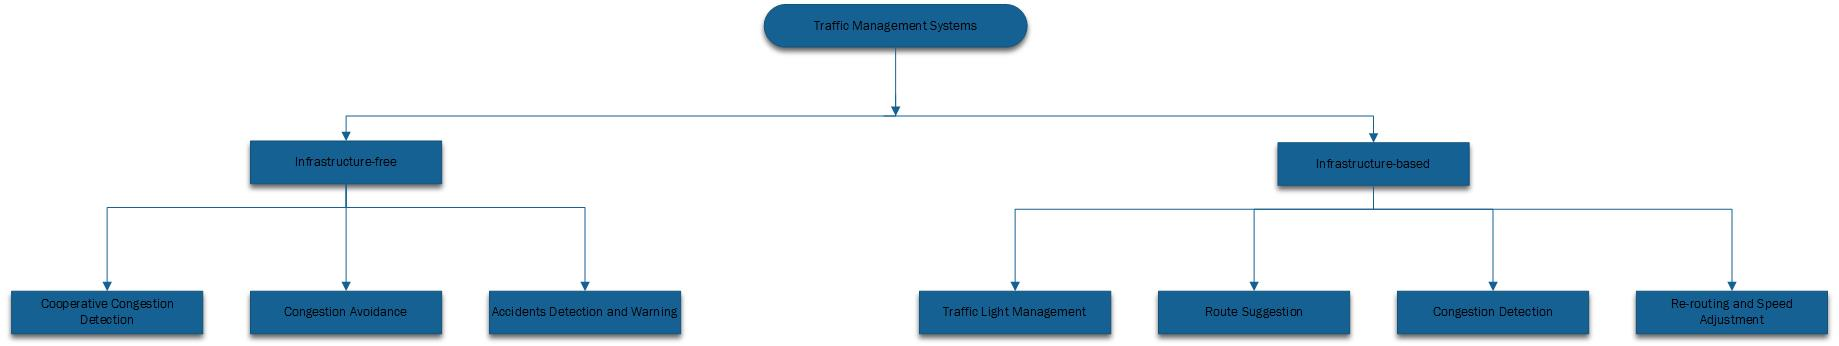
\includegraphics[width=7in]{flowDiagramTrafficManagement}
\caption{Traffic Management Systems Classification}
\label{flow_diagm}
\end{figure*}


 
 Traffic congestion is by no means a new problem. In our personal view smart traffic management system is all about urban traffic systems, safety, pollution and energy consumption. TMS is all about real-time data gathering and using that data to manage the traffic congestion.But it can be argued, obviously, we as of now have conveyed "smart" advancements for traffic management, we have CCTV cameras to monitor activity. Obviously, the CCTV frameworks permit some kind of vehicle distinguishing proof and even vehicle numbering utilizing which we can gauge conceivable regions of traffic blockage in a city in light of which city directors endeavor to take essential activities. 
 
 Be that as it may, then even with the CCTV frameworks sent, congested driving conditions are extremely regular is most urban areas and towns crosswise over Canada in a startling occasion of a street mishap or a vehicle separate. In such a startling occasion, the whole TMS appears to separate prompting to terrible movement clog affecting versatility of vehicle and walkers. 
 
 Thus, it is not generally comprehending the reason and expected purpose the fundamental objectives of a smart traffic management arrangement needs accurate data to accomplish feasible portability, and securing exact and opportune information about explorers developments to search for a streamlining of the accessible means it should be a smart sensor based wireless system centered in light of gathering real-time data on traffic with segments for, vehicle counting, vehicle, identification, monitoring noise levels, CO (carbon monoxide) and tidy levels,gases concentrations,humidity, etc.Since it is wireless, there would be no compelling reason to uncovered streets, embrace development works and have street terminations as a component of its organization. Thus, the general cost of organization is much lower and in actuality a fast and speedy arrangement is conceivable.

\subsection{Organization of the Survey}
The rest of this survey shall be organized in the following manner. In the next section, a brief technical background of TMS will be provided. This will lead into the definition of various metrics which may be employed in order to characterize advanced traffic management architectures. Afterwards, the contribution of other surveys in this field will be detailed such as to clarify the novelty of this one. The latest research delving into TMS in Internet of Things (IoT) are presented in the following sections and are broken down into sub-classes as shown in Figure \ref{flow_diagm}. It is pointed out that these sub-classes have received general consensus from researchers and have been adopted from previous surveys in the field \cite{souza:review}. Finally, these findings will be interpreted and discussed so to draw insight into the future of TMS.

\section{Background}

Based on the VANET, vehicles require two types of communication resources. The first resource includes vehicle to vehicle (V2V) that deals in communicating with other vehicles using Dedicated Short Range Communications (DSRC) and the later one vehicle to infrastructure (V2I) using long distance communication resource i.e.  LTE. 

Vehicles on road receive data from road sensors, traffic lights and other networks employing OBU modules and forward it to the vehicles of its short range. However, they can also transmit data to RSU using V2I resources through access network. The access network is in turn connected to the cloud with core network and this is how the core networks forward the data to cloud, thus the TMS implementation being enhanced. The whole TMS process generally takes three stages to complete its service of detecting traffic congestion: (i) Data Collection, which involves in assembling data from multiple sources (ii) Data operation, which entirely depends on combining data collected from diverse sources and process it further to check if there is any error which may eventually deteriorate the safety of TMS and (iii) User end service, the service provided to user by means of different multimedia service systems.

\textit{Data Collection} is a module or sensor that keeps collecting traffic oriented data from different origins covering vehicles, roadside sensors, incorporated device sensor such as GPS. The module OBU assembled these data to be shared with TMC. The road sensor especially the module RSU have the records of data history of traffic including the information of traffic light, traffic condition of roads etc. Furthermore, the web resource gives accurate information on traffic data such as posting and sharing on various types of social media has merged the traffic scenario and thus the traffic congestion being predicted.

\textit{Data Operation} enables traffic risk to be identified and estimated after executing the task of traffic information collection. For the TMS issue, it can be implemented both in infrastructure free and infrastructure-based system. In infrastructure-free system, vehicles share traffic risk information with other vehicles employing V2V technology which is distributed system. In the infrastructure-based, vehicles make proper use of main server such as TMC or other infrastructures in purpose of picking out the traffic risk information. It provides a better quality of  TMS service to people even if it has a long maintenance of greater amount of overhead compared to infrastructure free technology. 

\textit{User End Service} is provided to the user on account of identifying the traffic risk issues and avoiding the congestion. As per TMS theory, this service can be dispatched in both way infrastructure-free and infrastructure-based. Infrastructure free technology provides services including collision finding, collision avoiding which takes delay in response, whereas infrastructure-based technology offers better quality traffic management by providing the congestion identification, speed controlling and alternative way suggestion.

\subsection{Infrastructure-free TMS Taxonomy}
The pillars of Infrastructure-free TMS are as follows: 
\subsubsection{Cooperative congestion detection}
Enabling driver to react appropriately to changes in his immediate environment.
\subsubsection{Congestion avoidance}
V2V Communication  to streamline the operation of vehicles by overseeing vehicle movement, helping drivers with safety and sharing data, and in addition giving proper administrations to travellers.
\subsubsection{Accident detection and warning}
Occurrence cautioning projects are characterized as spacial projects, which build up a threat cautioning in reliance of the danger on the primary carriageway.



{
\tabulinesep=1mm
\begin{table}[!htb]
  \centering
  \begin{tabu} to 0.5\textwidth {|X[2,r]|X[6]|}
     \hline
      Collision warning&Cooperative forward collision warning, 
to be specific, to keep away from rear-end collisions \cite{adHocNetworks:Hartenstein}.\\\hline
      
      Wireless diagnosis &  Remote wireless diagnosis, in particular, to make the condition of the vehicle accessible for remote diagnosis\\\hline
      
     Signal synchronization & Traffic light ideal speed admonitory, to be specific, to help the driver to arrive during a green phase.\\\hline
     
     Efficacy and reliability & Where sender could misinterpret with falsely data to gain advantage. In this case a secured and authenticate network can secure the communication between vehicle in infrastructure-free TMS. \\\hline    
     Storage& We should note that in a system of vehicles, energy and storage space are adequately accessible. \\\hline
      
      
  \end{tabu}
  \smallskip
  \caption{Others factors in Infrastructure-free or V2V communications}
  \label{tab:V2Vmet}
\end{table}
}

\subsection{Infrastructure-based TMS Taxonomy}
The four sub-categories of Infrastructure-based TMS are summarized below and are visualized in Figure \ref{flow_diagm}.

\subsubsection{Traffic light management}
To identify the nearness of traffic waiting up at the light.
\subsubsection{Route suggest}
At the point when a specific street portion presents indications of congestion, the service searches for adjacent vehicles to re-route.
\subsubsection{Congestion detection}
Traffic management here is to distinguish and control clog by utilizing a decision-making algorithm which decides how the traffic light works in view of the data gathered from smart devices.
\subsubsection{Rerouting and speed management}
TMS regulate road traffic by sequencing traffic movements and setting routes with the aim of ensuring smooth transportation behavior and limiting, as much as possible, transport delays.




\begin{figure}[!ht]
\centering
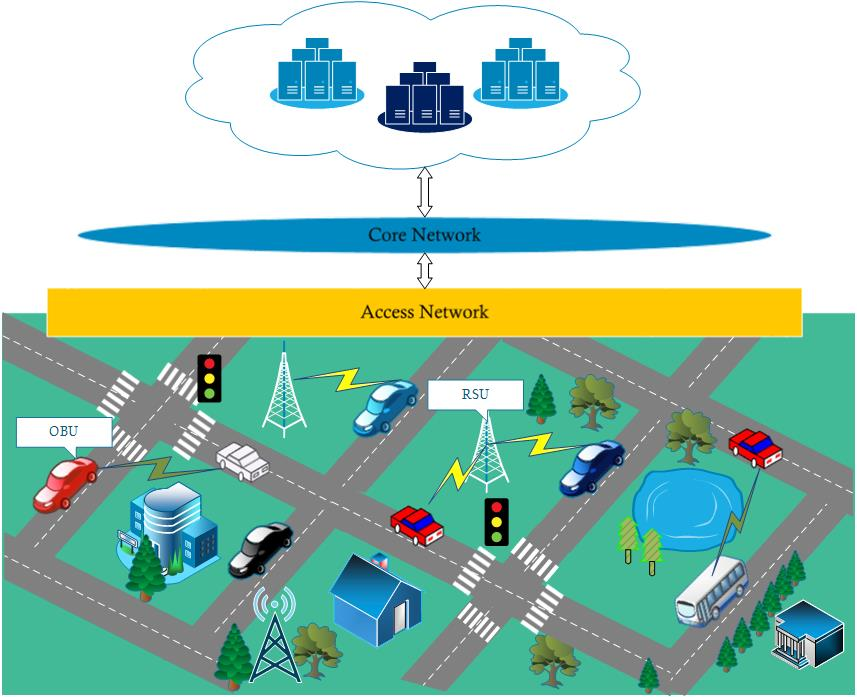
\includegraphics[width=3.5in]{wireless_traffice}
\caption{Over all TMS architecture}
\label{wireless}
\end{figure}



\section{Related Work}
Numerous surveys in the area of traffic management systems have been studied and considered a measurable extent for reducing the collision in roads, wait time of vehicles on traffic crossing points and emphasizing urgent vehicles.

We found a very comprehensive solution \cite{sanguesa2015sensing} while considering different natural conditions, for example, reduced light or unfavorable climate, enormously influence conventional strategies in view of infrastructure, e.g., ambient microphones or surveillance cameras.This ided is to collaborate the V2I and V2V technologies to enhance better solutions. Inductive loop detectors are not influenced by these issues, but rather the covered zone where they can evaluate vehicle density is constrained to the avenues where the information procurement devices are introduced, comparatively to past methodologies. Also, they need adaptation to internal failure, and communicate storm moderation systems can't be connected, since they are not ready to caution vehicles to change their dispersal policies. 

Density estimation plans in view of V2I communication give great capacities regarding control of movement blockage. Notwithstanding, their usefulness with respect to communicate storm decrease and adaptation to internal failure is constrained. For instance, in case of a RSU glitch, the density data of its secured zone couldn't be utilized for density estimation, since these information would not be accessible. The potential disappointments of this system (harmed infrastructure devices, backbone errors, and so forth.) can be overcome by utilizing \textit{Sanguesa et al.} \cite{sanguesa2015sensing} proposed V2X-d design.


{
\tabulinesep=1mm
\begin{table}[!htb]
 \centering
  \begin{tabu} to 0.5\textwidth {X[.9,r,c,m] X[0.4,c,m]  X[0.6,c,m] X[0.7,c,m] X[0.20,c,m] X[0.17,c,m] X[0.5,c,m] }
     \hline
     Features & Cameras & Loop Detectors & Microphones & V2I & V2V & V2X-d \\\hline

24/7 availability & \xmark & \checkmark & \checkmark & \checkmark & \checkmark & \checkmark \\\hline
Different Light condition & \xmark & \checkmark & \checkmark & \checkmark & \checkmark & \checkmark \\\hline
All sound condition & \checkmark & \checkmark & \xmark & \checkmark & \checkmark & \checkmark \\\hline
All weather condition & \xmark & \checkmark & \xmark & \checkmark & \checkmark & \checkmark \\\hline
Real time estimation & \xmark & \checkmark & \checkmark & \checkmark & \checkmark & \checkmark \\\hline
traffic jam avoidance  & \checkmark & \checkmark & \checkmark & \checkmark & \xmark & \checkmark \\\hline
Broadcast storm mitigation & \xmark & \xmark & \xmark & \xmark & \checkmark & \checkmark \\\hline
Fault tolerance & \xmark & \xmark & \xmark & \xmark & \checkmark & \checkmark \\\hline


      
      
  \end{tabu}
  \smallskip
  \caption{Comparison in density estimation}
  \label{tab:density}
\end{table}
}

Consolidating V2V and V2I interchanges permits diminishing the instability of the data accumulated and makes it as total as could be expected under the circumstances, in this way enhancing the general framework as far as blame tolerant abilities. 

A large portion of these issues can likewise be explained utilizing V2V approaches, yet the local information they give does not permit figuring ideal vehicle routes. Specifically, the data got by the vehicles is constrained to their neighboring vehicles, and the accessible density estimation is additionally restricted to their one-bounce scope territory. Their proposed V2X-d engineering consolidates the benefits of V2V and V2I approaches, conceding the likelihood of conveying new administrations for better activity control and decreased travel time and vehicle emanations \label{tab:density} shows their finding in different features. Specialists, transport offices and drivers will have the capacity to exploit these components to improve utilization of speedier and remote correspondence. A \$423m project on Intelligent Transport System (ITS) was carried to improve Hong Kong's busiest road transport network RoadTraffic\footnote{http://www.roadtraffic-technology.com/projects/hong-kong/}. The project was not easy to implement on hilly terrains so as to take longer time from 2001 to 2010. There were few initiative by US government in the Department of Transportation (DoT), Connected Vehicle Pilot Deployment Program. US government key point some important issues like Identify, develop, and deploy applications that leverage the trans-formative capabilities of wireless technology between
vehicles, infrastructure, and travelers’ personal communication devices to enable safer, smarter, and greener surface transportation solutions.This Proposal (RFP) released January 30, 2015. There was another exiting project called Illinois Tollway Drivers on the Illinois Tollway system are required to pay tolls as indicated by signs posted at toll plazas.

Drivers who pay cash may find themselves in an unattended toll plaza lane or in an I-PASS or Pay On line lane. If this happens, continue driving forward. Do not back up at any time it is unsafe. Make note of drivers location by identifying the toll plaza name or number or the nearest milepost. 

A driver will be required to identify the unpaid toll location when submitting your payment. Payments must be made within the 7-day grace period and can be made online or by mail. Jane Addams Memorial Tollway (I-90) - the rebuilt 16-mile ‘smart corridor’ used active TMS features to provide real-time information to drivers using a network of cameras, sensors and overhead electronic devices\footnote{https://www.illinoistollway.com/}.The key element it performed to identify congestion includes traffic data assembling, observing, data processing and controlling congestion. This project has enabled an effective TMS in important highways, underpass roads and branch roads.

Al-Holou \textit{et al.} \cite{al2012multi} proposed a traffic management model in which vehicles greatly relies on traffic clog, surrounding environment and traffic flow. His project deals with adaptive light controlling that minimize the traffic intensity and maximize the traffic flow using V2V/V2I technology. Christopher Davis \textit{et al.} project\footnote{http://www.citsm.umd.edu/documents/abstracts-finished/milner-abstract.php} implemented their project in University of Maryland focusing on the concept of high quality (HQ)digital video surveillance camera networked wirelessly . This project will enable efficient traffic analysis using better capturing HQ image and wireless network.

\section{Existing Infrastructure-free technology}
\subsection{Cooperative Congestion Detection}

Bauza \textit{et al.}\cite{bauza2013traffic} presented CoTEC (COperative Traffic congestion detECtion), a V2V communication based technology to identify traffic congestion assessed in large-scale broadway which accurately picks out and read the traffic congestion scenarios under different circumstances of traffic. Exchanging information through V2V or V2I communication, this technique enables road traffic information to be shared in a cooperative manner. Vehicles collaboratively determine the surrounding traffic condition periodically broadcast by vehicles and CoTEC makes it possible by applying CAMs (Cooperative Awareness Messages) which is also considered as beacon messages. CoTEC maintains the fuzzy-logic based algorithm while detecting traffic congestion using beacon signals gained from other vehicles. CoTEC performs a traffic congestion quatization process based on the fuzzy logic mechanism to segment the congestion. Collecting the traffic data from different sources needs fuzzy logic that is based on Level Of Service (LOS) found in Highway Capacity Manual (HCM) . LOS presents some operational statements while applying in the traffic flow. 

Araujo \textit{et al} \cite{araujo2014cartim} represented CARTIM (Cooperative vehiculAR Traffic congestion Identifi-
cation and Minimization), a proposal which employ V2V connection on purpose of detecting traffic congestion. Their simulation work proved CARTIM efficiently detect congestion and minimize it. CARTIM collaboratively estimates the traffic congestion level which is the same task as CoTEC does and both systems have decision making with the implementation of fuzzy-logic mechanism. However, the fuzzy logic rules, both systems are implementing are different from others since both rules are built in different matrices presented on HCM. This is how they are unlike in fuzzy logic mechanism. Moreover, CARTIM proposes a heuristic decision to change the way, thus minimizing the traffic density while detecting congestion. 




\subsection{Congestion Avoidance}
Meneguette \textit{et al} \cite{meneguetteenhancing} developed UNCONDES (Urban CONgestion Detection System) which involves in identifying traffic and reducing it in urban ares using V2V communication. Unlike the previous proposed model, UNCONDES is based on Artificial Neutral Network (ANN) to detect traffic congestion problem and it represents the dimension of traffic congestion, thus suggesting the  alternative route to avoid congestion. This is how this technology also decrease the amount of fuel consumption. ANN implemented in UNCONDES collects the data of speed and density of routes and it is done by receiving the beacons of all vehicles plying on the roads periodically \cite{yousefi2006vehicular}. The input parameter configured in ANN uses the data of vehicle speed and its density on roads and the congestion level of road used as output. ANN classifies the output into three levels of congestion \cite{meneguetteenhancing}. They are: 

Free: output is lower or equal to 0.3

Moderate: when the output is in between 0.3 and 0.7

Congested: Output is above or equal to 0.7


This is how a vehicle gets beacon messages from surrounding vehicles that contains data of classification level of congestion and based on that message it checks if it can pass the roads. If it finds congestion, then it follows the mechanism to avoid this route and get suggestion to take alternative pathway having less congestion.
\subsection{Accident Detection and Warning}
Souza \textit{et al.} \cite{de2016fully} proposed a fully distributed V2V communication based TMS, FASTER that develops the traffic efficiency by gathering the exact data of traffic for each vehicle. Based on this purpose, FASTER enables all vehicles acquire information of traffic scenarios and disseminate it to other neighbors. Therefore, the knowledge of traffic data is to be developed. To ease the execution, FASTER chunk  the whole scenarios in segments, named Districts on purpose of developing the knowledge of traffic in that particular division.  Moreover, roads under each district contain overall knowledge of road traffic density and speed of vehicles.  In this way, the district based information of traffic is shared with other vehicles through disseminating beacons. Due to the rapid changes of vehicle density and network architecture continual changes, VANET faces a limitation in employing data dissemination protocols, thus decreasing the dissemination capacity. This limitation is \textit{broadcast storm problem} \cite{souza2014add} that occurs especially when multiple vehicles plying on road try to transmit at the same time. FASTER has the ability to overcome this problem. Moreover, it has the mechanism to overcome the obstacles of \textit{resynchronizing effect} \cite{souza2014add} developed by IEEE 802.11p. After receiving all the knowledge of district, vehicles develop a graphical relation G=(V,E), where V is a set of crossing points and E is a set of routes that represent the scenerio. Moreover, each road carries a weight focusing on the average speed of vehicles on road. Hence, FASTER allows each vehicles to have exact information of traffic condition.
Souza \textit{et al.} \cite{Souza:2014:DGE:2642668.2642677} proposed a TMS based on inter-vehicle communication system which avoids the highly dense route and shorten the travel time, consequently lessen the fuel intake and spread of CO2 emission. To overcome the broadcast storm problem, this model implements DRIFT algorithm which increases the data disseminating capacity with low over head, thus disseminating the warning data of accident.

A fully-distributed, pro-active TMS, GARUDA (Geographical Accident aware to Reduce Urban Congestion) was founded by Souza \textit{et al.} \cite{de2015garuda} to reduce the congestion level in urban areas. GARUDA implements in three stages: (i) Information Generation (ii) Information Dissemination and (iii) Making Real Time Decision. \textit{Information Generation}: During mishap, the running vehicles share an alarm message with other forwarding vehicles to make them aware of the geographical coordinates of occurrence. In GARUDA, an OBD 2 system (On Board Diagnostic 2) is required to determine the real time information of vehicles, such as, speed and air bag status etc.Thus, GARUDA is able to detect the accident and pass this message to the next module. \textit{Information Dissemination}: During the disseminating stage, GEDDAI-NP (Geographical
Data Dissemination of Information and Alert Aware of Network
Partition) protocol is used to spread the message over network. Consequently, it circumvents the obstacles of broadcast storm problem, thus making short delay with low overhead and increasing the efficiency of disseminating capacity. \textit{Making Real Time Decision}: As soon as the alarm message being received, a decision of short delay is made using the \textit{Making Real Time Decision} module in application segment. Using this module, vehicles check if the accident location is suitable to pass. If not possible then a new route is suggested to avoid the accident place.








\begin{figure}[!ht]
\centering
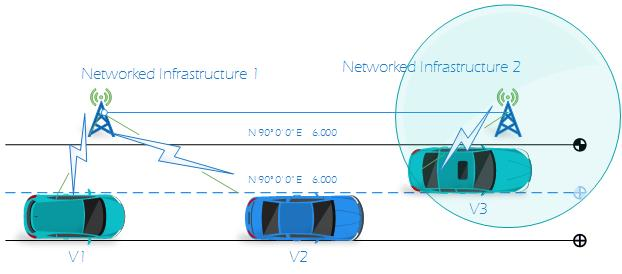
\includegraphics[width=3.5in]{V2I}
\caption{Vehicle to Infrastructure TMS}
\label{fig_ldosAttProf}
\end{figure}

\section{existing infrastructure-based technology}
\subsection{Traffic Light Management}
Rakha \textit{et al.} \cite{rakha2011eco} came up with a V2I communication based model, a traffic light management system that is built in traffic crossing point for  intelligent Traffic Light (ITLs). It reduces the amount of time vehicles waste on traffic light intersection, thereby fuel is efficiently utilized which in turn limit the release of CO2. To  retain fuel  utilization in an  optimum level, each  vehicle  regulates  its  speed. Consequently, they don't have to wait long time on the traffic light intersection. To accelerate this process, this eco-driving model transmits data to the  vehicles in coverage  area  approaching towards the traffic light intersection. These data represent vital information such as, traffic  light current situation,  the  timing  to  the subsequent stage and,  the span  of  vehicles’ serial  at  the intersection  called  SPaT  (Signal  Phasing  and  Timing). Eventually, based on obtaining a SPaT information, the vehicles calculate the instantaneous  optimum velocity by means of the VT-Micro model which computes the fuel utilization  for  a number of  different  speed  profiles to verify which is the optimum.

Wei-Hsun Lee \textit{et al.} \cite{lee2012decision} developed a V2I based system, DTGDSS (Decision-Tree  based  Green  Driving  Suggestion  System) focusing on the purpose of limiting the carbon emission and at the same time it recommends the best economic routes to the vehicles. In DTGDSS system, RSU, employed in traffic light is connected to vehicles and have the proper data of velocity, location and direction sent by vehicles. As soon as RSU receives data, it computes the density or the span of line of each direction at the crossing-point which can be extracted through differentiating its location with the last stopped vehicle in the line of each direction. In this way, when a RSU shares the data of traffic condition, length of vehicle line at intersection to vehicles, it compute its speed and adjust in such a way that lessen the waiting queue length and maximize throughput.


\subsection{Route Suggestion}
Pan \textit{et al.} \cite{pan2012proactive} considered three re-routing techniques to be applied in economic traffic guidance system. This system enables the vehicle to receive traffic data and take actions to change the route in response to the acquired instructions. A centralized traffic monitoring and re-routing service, a vehicle software stack for producing periodic traffic data reporting(position, speed, direction) are included in this guidance system. Moreover, this system executes in 4 stages that are performed sequentially: (1) data acquisition and representation; (2) traffic congestion identification; (3) vehicle selection
for re-routing; and (4) alternative route estimation.  
Traffic data is acquired and represented through a directed graph where the nodal points refer to crossing-point and edges refer to the road sections, and weight is considered as computed travel time. In the identification stage, the service checks the congestion in road section periodically. Next stage is re-routing stage where the service enables re-routing to another closer vehicle if it finds any congestion in road. Estimating alternative route involves calculation of the alternative route to formerly selected vehicles. 
In addition, alternative route calculation requires 3 different strategies: (i) Dynamic Shortest Path (DSP) is the traditional re-routing strategy that selects the vehicles to the destination path of lowest travel time. It seems to be good when the amount of re-routed vehicle is not higher, but it may not work well for higher re-routed vehicle. (ii) Random k Shortest  Paths (RkSP) calculates k shortest path for each vehicle and allocates the vehicle to one of them randomly to decrease the congestion of another area, the limitation of DSP (iii) Entropy  Balanced k Shortest  Paths  (EBkSP) balances the traffic by computing k shortest paths for each
vehicle and set the selected vehicle to the path with the lowest popularity as proposed by the path entropy. 

To enable the congestion detection and balancing traffic, a systematic flow control mechanism was deployed by Brennand \textit{et al.} \cite{brennand2015intelligent} where they noticed a V2I communication based ITS that detects and reduce the traffic congestion with keeping the traffic flow in an optimum level, thus making the travel time shorter and consequently intake of fuel is limited to establish less carbon emission. The proposed system consists of RSUs disributed over the whole architecture that enable the congestion detection and balancing traffic. In details, the system is comprised of (i) RSU distribution over whole network (ii) Data gathering; and (iii)  Congestion detection and control. RSU distribution depends on the communication range of RSU, and the measurement of maps and focuses on how much it can cover the whole map with the minimum  number of RSUs.  RSU receives the information (location, velocity, present route, direction and the average time they took to move through each road in their route) from the nearby vehicles within its coverage range which is done with the single-hop long-range communication system, such as 3G or LTE. With the information provided by the vehicles, RSU perceive the condition of the area covered within its communication range and then represent a graph besed on the received information. The graph is represented by G = (V,E), where V is the set of intersections and E is the set of road sections of each RSU communication radius \cite{souza:review}. Roads in the graph G represent a weight referred to the estimated velocity of vehicles and maximum allowable velocity. Moreover, the weight is inversely proportionate to the velocity at which vehicles move through the road. In addition to graphing, RSU enables re-routing to each vehicle periodically within its range till each vehicle can travel the congestion free path. Re-routing occurs from the present location of vehicle to the last road vehicle will reach the destination. RSU takes the splitting route of the vehicles where they travel and computes the k shortest paths, consequently it finds the alternative paths. Eventually, RSU extracts the best alternative path from these paths using the Boltzamann  probability distribution \cite{kirkpatrick1983optimization} and rest of the paths are adjusted to the new route calculation and send it to the vehicles.
\subsection{Congestion Detection}

Younes \textit{et al.} \cite{younes2013efficient} proposed a congestion detection protocol, ECODE  (Efficient  road COngestion  DEtection  protocol) to detect the high volume of traffic in the road segment along with its direction which can be applied either V2V or V2I communication system. In their proposed system, inter-vehicle communication was enabled through the advertisement message (ADV) carrying vehicle's ID, velocity, position, destination, direction of vehicle, occurrence time with the use of multi-hop data communication that follows the geocast principles. Upon receiving the ADV, each vehicle combines it into the Neighbors Report (NR) and in turn, they send the Traffic Monitoring Report  (TMR) to the nearest RSU that contains the information of traffic volume, average travel time, average speed on the road. After having TMR on database of RSU, it scrutinizes and find the best path for each destination. Finally, it provides the \textit{RecomReport} messages in response to the vehicles which comprise the data of ID, best roundabout route, TMR and travel time. In this way, the vehicle becomes able to calibrate its route to the destiation and pass this message to other nearby vehicles.

Pan \textit{et al.} \cite{pan2017divert} came up with a different approach and their proposed name is DIVERT, a distributed vehicular re-routing system for congestion repudiation that unload the segment of re-routing configuration that is exceptionally good in preserving the users privacy and providing the real time congestion avoidance. To accomplish this process, using a data server is must for vehicles to obtain the comprehensive traffic data. Moreover, the data server keeps sending notification to the vehicles as soon as it finds out any congestion and the vehicles, in turn, share this information with other neighboring vehicles over vehicular ad hoc networks. In this way, vehicles can identify if they can pass through the congestion. If not possible, they re-route themselves collaboratively to omit congestion and maintain a better traffic.




\subsection{Re-routing and Speed Adjustment}
Doolan and Muntean found an innovative approach, EcoTrec, which aims to decrease the amount of carbon emission providing with compromising the travel time of vehicle hence this approacher suggest a better routing algorithm technique build a fuel efficiency model of the routes. On their proposed model the main issues they focused on greenhouse effect as well as global warming this is what outcomes show in their result of EcoTrec project \cite{doolan2016ecotrec}.

Wang \textit{et al.} introduced Next Road Rerouting (NRR) \cite{7385577}, an adaptive re-routing technique to reduce the unexpected traffic congestion. It utilizes the local information stored in RSU established at each crossing-point on purpose of selecting the best route. In this way, this system saves the expenses for securing the global traffic knowledge. Each RSU obtains the local information through the beacon messgaes disseminated by the vehicles. Moreover, RSU uses Traffic Operation Center (TOC)  for identifying the congestion of its nearest location where TOC sends congestion information to the RSU adjucent to congestion and RSU, in turn, broadcasts it to the vehicles within its coverage area. Consequently, the vehicles become  updated with the latest traffic information and keep verifying if it can pass through the congestion.






\section{Interpretation and Discussion of Findings}

It was found that the infrastructure free classifications adopted from \cite{souza:review} are still relevant in regards to recent findings. That is, no new research in the field constitutes a brand new category. This does not come as a surprise due to the maturity of studies in TMS.Furthermore, it was found that most advances in TMS stem\cite{Multimedia:chao}  is related to multimedia devices in RSU and OBU.

In the case of technologies, a wealth of information was revealed by the literature review of this survey. It is noted that purely source end solutions have not been as recently active as other categories.The surveyed mechanisms expand on, and optimize, existing techniques and others make use of paradigms with growing popularity and management technique in TMS.

%TODO



\section{Conclusions}
In this paper, we briefly discussed traffic management systems  before presenting a classification and taxonomy inspired by previous surveys in the field for both infrastructure-free and infrastructure-based mechanisms. We then introduced recent research papers on the subject of infrastructure-free targeting the V2V communications, followed by infrastructure-based techniques collaborating with V2I technique, all of which we classified and characterized following our taxonomy. Finally, we interpreted and discussed our findings.

Though infrastructure-based communication is a very mature field and research in the area is abundant, it is still in evolution and problems still remain unsolved. Infrastructure-free techniques are making great advances, becoming more and more effective and sophisticated as we have shown, but the effectiveness of even the most recent research such as the one traffic solution\footnote{https://www.swarco.com/en/Products-Services/Traffic-Management/Urban-Traffic-Management/Urban-Traffic-Systems} demonstrate that work still needs to be done in that regard.

\bibliographystyle{ieeetr}
\bibliography{papers.bib}
% use section* for acknowledgment
%\section*{Acknowledgment}
\end{document}